\section{Strumenti}
\subsection{Alberi di Merkle}

Gli alberi di Merkle sono una particolare struttura ad albero che sfrutta le proprietà delle funzioni di Hash al fine di
ottimizzare le operazioni di ricerca e identificazione delle modifiche all'interno della collezione. La struttura degli
alberi di Merkle è composta dalle foglie, che rappresentano i dati a cui è stata applicata una funzione di
hash e dai nodi, che sono ottenuti uno dopo l'altro applicando la funzione Hash ai loro figli, fino a raggiungere
la radice. Negli alberi di Merkle la radice è una funzione Hash che rappresenta univocamente la struttura. Per capire
meglio il concetto immaginiamo di avere un struttura ad albero binaria, e inseriamo all'interno della struttua gli
elementi 1,2,3,4,5 a cui applichimao una funzione Hash, a questo punto otterremo la seguente struttura:
\begin{figure}[H]
    \centering
    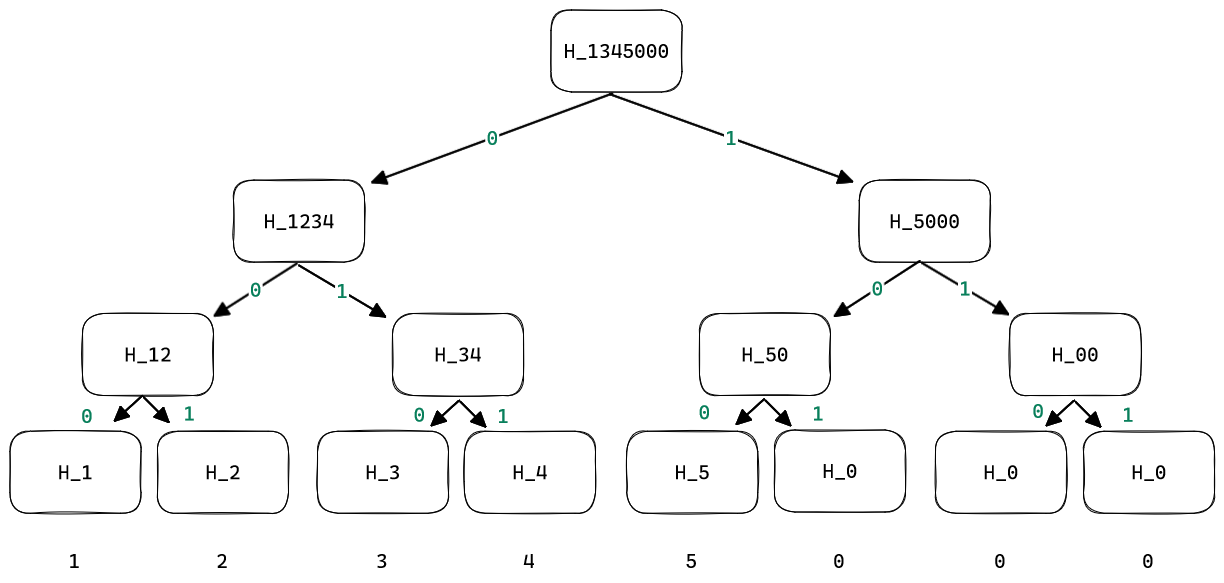
\includegraphics[width=13cm]{./chapters/2.rln-protocol/images/1.merkle_tree.png}
    \label{fig:merkle_tree}
    \captionsetup{justification=centering}
    \caption{Esempio struttura albero di Merkle binario}
\end{figure}
Possiamo notare che la radice degli alberi di Merkle possiede la proprietà di essere una sorta di impronta digitale
della struttura, in quanto qualsiasi modifica ai dati comporterebbe un cambiamento a cascata dei nodi fino alla radice
stessa. Questa proprietà costituisce un vantaggio significativo in termini di efficienza. Infatti, consente una verifica
rapida delle modifiche apportate alla struttura, rendendo gli alberi di Merkle estremamente utili nei campi
decentralizzati e nei file system condivisi, dove l'individuazione efficiente dei cambiamenti con poche informazioni è
cruciale. Un'altra proprietà altamente utile degli alberi di Merkle è la loro capacità di verificare l'appartenenza di
un elemento alla struttura in modo efficiente e senza la necesità di conoscere l'elemento in chairo. Nell'esempio
precedente, se si desidera verificare che l'elemento 4 appartenga alla struttura, è sufficiente utilizzare gli elementi
H\_3, H\_12 e H\_5000 e il valore H\_4, che non rivela alcuna informazion su l'elemento. Una volta ottenuta la radice
basterà confrontarla con la radice corretta per convicersi della presenza dell'elemento o meno nella struttura.
\begin{figure}[H]
    \centering
    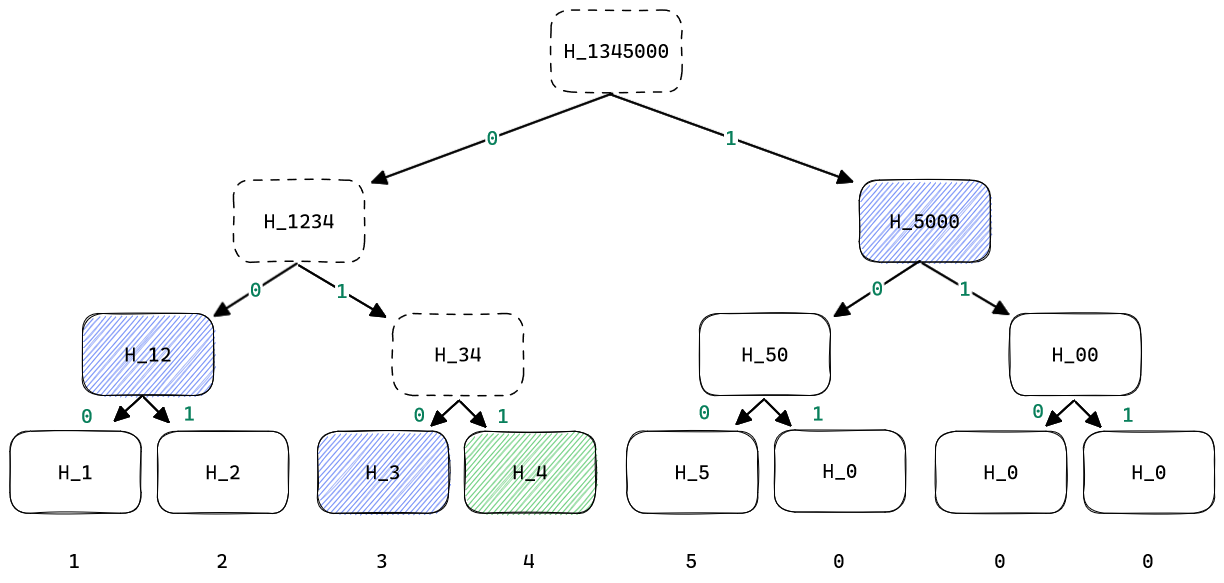
\includegraphics[width=14cm]{./chapters/2.rln-protocol/images/2.merkle_proof.png}
    \label{fig:merkle_proof}
    \captionsetup{justification=centering}
    \caption{Esempio Merkle proof}
\end{figure}
Questo processo viene chiamato "Merkle proof" o più in generale "proof of membership". Tale processo rappresenta
l'approccio che adotteremo per dimostrare la capacità di un utente già registrato e non rimosso di interagire con il
sistema nella fase di Interazione del protocollo RLN.

\subsection{Nuove funzioni di Hash}
Indubbiamente, una delle tecniche più utilizzate in crittografia sono le funzioni di Hash. Anche la tecnologia zk-SNARK
non può fare a meno di esse. Infatti, come abbiamo già visto in molte situazioni, l'utilizzo di metodi di hashing è
stato necessario per ridurre le dimensioni delle informazioni e per nasconderle.Tuttavia, quando si utilizzano le
tradizionali funzioni di Hash come la versione Sha-256 nel campo delle Zero Knowledge proof, si verifica un problema.
Queste funzioni non sono state concepite per lavorare in domini di campi finiti e, pertanto, sfruttano metodologie come
la ripetizione di operazioni bit-wise, che tendono se trasforamte con R1CS ad aumentare considerevolmente la dimensione
dei vincoli del circuito. Questo aumenta notevolmente il tempo e la dimensione richiesti
per generare le prove. Negli ultimi anni, per superare il problema descritto, sono state utilizzate nuove versioni di
funzioni Hash come Pedersen, Rescue-$x^5$ e Poseidon. Queste funzioni sono state progettate specificamente per lavorare nei
campi finiti e con l'obiettivo di ridurre al minimo i tempi di generazione e i vincoli necessari per costruire le prove.
Tra queste funzioni, la funzione Poseidon è quella che ha ottenuto i risultati migliori e che verrà utilizzata nella
costruzione del circuito per il protocollo RLN. Di seguito vengono mostrate delle tabelle contenteti un confronto delle
prestazioni tra le più note funzione di Hash per le tecnologie Zero Knowledge e la funzione Sha-256, tabelle tratte da
"POSEIDON: A New Hash Function for Zero-Knowledge Proof Systems" \cite{cryptoeprint:2019-458}. Nelle tabelle sottostanti
possiamo notare che ci sono diverse configurazioni della funzione Poseidon. Infatti, una grande differenza tra le
funzioni tradizionali e Poseidon è la possibilità di scegliere il numero di iterazioni e la dimensione del campo finito
su cui lavorare, in modo da selezionare la versione più performante a seconda del caso.\\
\begin{figure}[H]
    \centering
    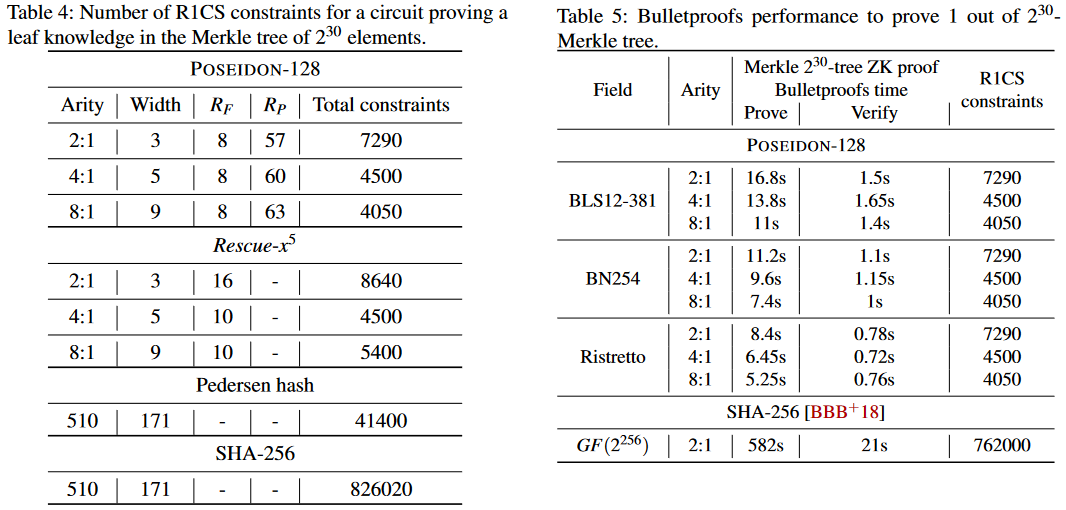
\includegraphics[width=14cm]{./chapters/2.rln-protocol/images/3.poseidon_comparison.png}
    \label{fig:poseidon_comparison}
    \captionsetup{justification=centering}
    \caption{Confronto con altri algoritmi Hash}
\end{figure}

\subsection{Nullifier}
I "nullifier" in crittografia sono dei valori utilizzati per confermare o annullare operazioni. Nelle applicazioni che garantiscono
l'anonimato, questi valori vengono spesso utilizzati per evitare il problema del "double-signaling", ovvero impedire che
un utente utilizzi o esegua un'operazione che dovrebbe essere unica per ogni utente più di una volta. Questo problema
può verificarsi perché, in assenza di un collegamento tra i dati e le identità degli utenti, non è possibile verificare
se un utente ha già effettuato o completato una determinata operazione. Ad esempio, in un'applicazione elettorale è
importante impedire che un singolo elettore voti più di una volta, mentre nel campo delle criptovalute è fondamentale evitare che la
stessa moneta, venga spesa più volte. Il problema si risolve utilizzando i nullifier ovvero valori univoci legati
all'operazione che riamangono privati fino al momento dell'effetuazione dell'eoperazione e una volta attauta vengono
resi pubblici, e salvati in modo da poterli consultare successivamente.
\begin{figure}[H]
    \centering
    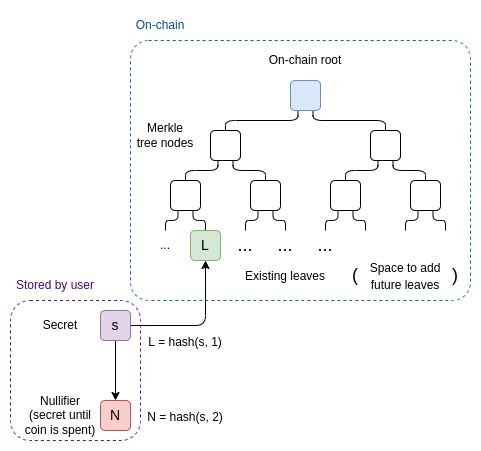
\includegraphics[width=10cm]{./chapters/2.rln-protocol/images/4.nullifier.png}
    \label{fig:nullifier}
    \captionsetup{justification=centering}
    \caption{Rappresentazione della creazione di un nullifier, tratta da \cite{some-ways-to-use-zk-snarks-for-privacy}}
\end{figure}
Dalla descrizione fornita potrebbe subito venire in mente il concetto di "rate-limiting" e si potrebbe pensate di
utilizzare i "nullifier" per attuare questa procedura in modo anonimo. In effetti, è possibile limitare gli
utenti utilizzando questa metodologia, pero non si potrà rivelare l'identità dell'utente malintenzionato che, in questo
modo, potrebbe riprovare indisturbato ad attacare il sistema.